\chapter[Relativistic EM]{Relativistic formulation of electromagnetism}
\section{Charge invariance}
Let us now discuss the formulation of electromagnetism in the relativistic framework. First off we start with stating a property:
\begin{quotation}
  The charge of a particle is independent of its velocity, thus it is Lorentz invariant
\end{quotation}
This makes sense since Maxwell's equations (in contrary to Newton's equations) are already Lorentz invariant.\\
As an example we take a volume $V$ at rest in an IRF $\irf{R}$ that contains $N$ elementary particles of charge $e$. The total charge inside the volume is:
\begin{equation}
  Q = Ne
\end{equation}
But we can also describe the total charge in terms of the charge density $\rho$:
\begin{equation}
  Q = \rho V = n e V
\end{equation}
Where $n$ is the number of charges per unit volume in the reference frame. If we take a second IRF $\irf{R}'$ in motion with respect to the first one we have:
\begin{equation}
  Q' = \rho'V' = n'eV'
\end{equation}
Since we stated that the total charge must be the same in all IRFs we have:
\begin{equation}
  n e V = n'eV'
\end{equation}
We have that the volume transforms as $V' = \dfrac{V_0}{\gamma(v)}$ where $V_0$ is the volume measured at rest which means that $V = V_0$. Thus we get:
\begin{equation}
  \begin{split}
    n \cancel{V_0} &= n' \dfrac{\cancel{V_0}}{\gamma(v)} \\[8pt]
    n' &= n\gamma(v)
  \end{split}
\end{equation}
This means that we see more charges per unit volume in the moving IRF, which makes sense if we think that the number of charges is the same but the volume is ``squeezed'' by the effect of lenght contraction.\\ The same is true for the charge density:
\begin{equation}
  \boxed{\rho' = \rho_0 \gamma(v)}
\end{equation}
Where $\rho_0$ is the proper charge density, measured in the IRF where the volume is at rest. We can also notice that $\rho$ transforms as $\diff{x^0}$.\\
The infinitesimal charge is also invariant and so also the following quantity is invariant:
\begin{equation}
  \diff{q} = \rho \diff{V}
\end{equation}
But also the infinitesimal volume in 4 dimensions is invariant, in fact we just have that:
\begin{equation}
  \diff{^4x} = \diff{x^0}\diff{x^1}\diff{x^2}\diff{x^3}
\end{equation}
Which transforms with:
\begin{equation}
  \diff{^4x'} = \det \lm \diff{x'^0}\diff{x'^1}\diff{x'^2}\diff{x'^3}
\end{equation}
The determinant of the Lorentz matrix is essentially the contribution of the Jacobian in any change of variable, but we previously got that the determinat of the Lorentz matrix is $1$ so:
\begin{equation}
  \diff{^4x'} = \diff{^4x}
\end{equation}
\section{Potentials}
We need to define a current density tensor. Could $J^{\mu} = \brackets{\rho, \vec{J}}$ be a good candidate? The answer is no, since the tensor would have quantities of different dimensions, but it turns out that $J^{\mu} = \brackets{\rho c, \vec{J}}$ works just fine as we will now see.\\
We have:
\begin{equation}
  J^{\mu} = \brackets{\rho c, \vec{J}} = \brackets{\rho_0 \gamma(v) c, \rho_0 \gamma(v) \vec{v}} = \rho_0 \gamma(v)\brackets{c, \vec{v}} = \rho_0 \gamma(v)u^{\mu}
\end{equation}
This seems good. If we do this the continuity equation can be reduced to a very simple and elegant form:
\begin{equation}
  \begin{split}
    &\div{\vec{J}} + \pdv{\rho}{t} = 0 \\[8pt]
    &\pdv{J_x}{x} + \pdv{J_y}{y} + \pdv{J_z}{z} + \pdv{\brackets{c\rho}}{\brackets{ct}} = 0 \\[8pt]
    &\partial_{x^1}J_{x^1} + \partial_{x^2}J_{x^2} + \partial_{x^3}J_{x^3} + \partial_{x^0}J_{x^0} = 0
  \end{split}
\end{equation}
This can be written in the compact form:
\begin{equation}
  \boxed{\partial_{\mu}J^{\mu} = 0}
\end{equation}
Now we are ready to define our new potentials. When we discussed about electromagnetism we got these equations:
\begin{equation}
  \begin{split}
    &\dalop \potE = -\dfrac{\rho}{\epsz}\\[8pt]
    &\dalop \vec{A} = -\muz \vec{J}
  \end{split}
\end{equation}
It can be shown that D'Alembert operator is Lorentz invariant. Now we want again a compact form for the equations of the potentials. Let's try to get again the quantity $\rho c$. In the first equation we have:
\begin{equation}
  \begin{split}
    &\dalop \potE = -\dfrac{\rho}{\epsz}\\[8pt]
    &\dalop \dfrac{\potE}{c} = -\dfrac{\rho c}{\epsz c^2}\\[8pt]
    &\dalop \dfrac{\potE}{c} = -\epsz \muz \dfrac{\rho c}{\epsz}\\[8pt]
    &\dalop \dfrac{\potE}{c} = -\muz \rho c
  \end{split}
\end{equation}
So we can define a tensor:
\begin{equation}
  A^{\mu} = \brackets{\dfrac{\potE}{c}, \vec{A}}
\end{equation}
Which allows us to write all the potential equations in the compact form:
\begin{equation} \label{e:potential_first_step}
  \dalop A^{\mu} = -\muz J^{\mu}
\end{equation}
This can be further simplified if we think about the definition of the D'Alembert operator:
\begin{equation}
  \begin{split}
    &\dalop = \partial_x^2 + \partial_y^2 + \partial_z^2 - \underbrace{\dfrac{1}{c^2} \partial_t^2}_{\frac{\partial^2}{\partial\brackets{ct}^2}} \\[8pt]
    &\dalop = \partial_{x^1}^2 + \partial_{x^2}^2 + \partial_{x^3}^2 - \partial_{x^0}^2
  \end{split}
\end{equation}
If we expand the second derivative and lower an index we get:
\begin{equation}
  \begin{split}
    \dalop = \partial_{x^1}\partial_{x^1} + \partial_{x^2}\partial_{x^2} + \partial_{x^3}\partial_{x^3} - \partial_{x^0}\partial_{x^0} \\[8pt]
    \dalop = -\partial_{x^1}\partial^{x^1} - \partial_{x^2}\partial^{x^2} - \partial_{x^3}\partial^{x^3} - \partial_{x^0}\partial^{x^0}
  \end{split}
\end{equation}
And so \eqref{e:potential_first_step} becomes:
\begin{equation}
  \boxed{\partial_{\mu}\partial^{\mu} A^{\mu} = \muz J^{\mu}}
\end{equation}
We can also write the equations of the potentials in integral form with tensor notation. For $\potE$ we have:
\begin{equation}
  \begin{split}
    &\potE = \dfrac{1}{4 \pi \epsz}\int \dfrac{\rho \brackets{t- \dfrac{\norm{\vec{r}-\vec{r}'}}{c}}}{\norm{\vec{r}-\vec{r}'}}\diff{^3 \vec{r}'} \\[8pt]
    &\dfrac{\potE}{c} = \dfrac{1}{4 \pi \epsz c^2}\int \dfrac{\rho c \brackets{t- \dfrac{\norm{\vec{r}-\vec{r}'}}{c}}}{\norm{\vec{r}-\vec{r}'}}\diff{^3 \vec{r}'} \\[8pt]
    &A^0 = \dfrac{\muz}{4 \pi}\int \dfrac{J^0\brackets{t- \dfrac{\norm{\vec{r}-\vec{r}'}}{c}}}{\norm{\vec{r}-\vec{r}'}}\diff{^3 \vec{r}'}
  \end{split}
\end{equation}
The other components $A^1, A^2, A^3$ are already in this form so we have:
\begin{equation}
  A^{\mu} = \dfrac{\muz}{4 \pi}\int \dfrac{J^{\mu}\brackets{t- \dfrac{\norm{\vec{r}-\vec{r}'}}{c}}}{\norm{\vec{r}-\vec{r}'}}\diff{^3 \vec{r}'}
\end{equation}
\section{Gauge transformations}
Recalling that Gauge transformations are:
\begin{equation}
  \begin{split}
    &\potE \longrightarrow \potE' = \potE - \pdv{\xi}{t} \\[8pt]
    &\vec{A} \longrightarrow \vec{A}' = \vec{A} + \grad{\xi} \\[8pt]
  \end{split}
\end{equation}
The first equation can be reduced in tensor notation by simply dividing by $c$:
\begin{equation}
  \begin{split}
    &\dfrac{\potE'}{c} = \dfrac{\potE}{c} - \pdv{\xi}{\brackets{ct}}\\[8pt]
    &A'^0 = A^0 - \partial_0\xi \\[8pt]
    &A'^0 = A^0 - \partial^0\xi
  \end{split}
\end{equation}
We needed to raise an index since we cannot sum covariant quantities with contravariant ones. Now, the second equation is almost in the form we want, but we still need to raise the indeces:
\begin{equation}
  \begin{split}
    &\vec{A}' = \vec{A} + \grad{\xi} \\[8pt]
    &A'^k = A^k + \partial_k\xi \\[8pt]
    &A'^k = A^k - \partial^k\xi
  \end{split}
\end{equation}
In this case raising an index changes sign since $k=1,2,3$. So we can finally write Gauge transformations in tensor notation:
\begin{equation}
  A'^{\mu} = A^{\mu} - \partial^{\mu}\xi
\end{equation}
\subsection{Lorenz gauge}
We defined the Lorenz gauge such that:
\begin{equation}
  \div{\vec{A}} +\dfrac{1}{c^2}\pdv{\potE}{t} = 0
\end{equation}
We can easily write this in tensor notation:
\begin{equation}
  \begin{split}
    &\div{\vec{A}} +\dfrac{1}{c^2}\pdv{\potE}{t} = 0 \\[8pt]
    &\partial_1A^1 + \partial_2A^2 + \partial_3A^3 +\pdv{\dfrac{\potE}{c}}{\brackets{ct}} \\[8pt]
    &\partial_1A^1 + \partial_2A^2 + \partial_3A^3 + \partial_0A^0
  \end{split}
\end{equation}
Which leads to:
\begin{equation}
  \boxed{\partial_{\mu}A^{\mu} = 0}
\end{equation}
We can observe that this is very similar to the equation of the conservation of charge $\partial_{\mu}J^{\mu} = 0$.\\
If we are already in the Lorenz gauge and we want to remain inside the Lorenz gauge the condition that $\xi$ must obey was previously derived to be:
\begin{equation}
  \begin{split}
    \dalop \xi = 0 \\[8pt]
    \partial_{\mu}\partial^{\mu}\xi = 0
  \end{split}
\end{equation}
\section{The electromagnetic tensor}
If we look back at the problem with the wirte that we analyzed in the section about electromagnetism, we can understand that electric fields can become magnetic fields and viceversa if we change the IRF. This phenomenon can be explained using tensors. Let's remember that the electric field's general definiton is:
\begin{equation}
  \vec{E} = -\grad{\potE} - \pdv{\vec{A}}{t}
\end{equation}
Let us write the $x$ component of the electric field:
\begin{equation}
  \begin{split}
    E_x &= -\partial_x \potE - \pdv{A_x}{t} \\[8pt]
    \dfrac{E_x}{c} &= -\partial_x \dfrac{\potE}{c} - \pdv{A_x}{\brackets{ct}} \\[8pt]
    \dfrac{E_x}{c} &= -\partial_1 A^0 - \partial_0 A^1 \\[8pt]
    \dfrac{E_x}{c} &= \partial_0 A_1 - \partial_1 A_0
  \end{split}
\end{equation}
This can be seen as the element of a matrix in position $(0,1)$. We can thus define the \textbf{electromagnetic tensor}:
\begin{equation}
  F_{\mu\nu} \defineeq \partial_{\mu}A_{\nu} - \partial_{\nu}A_{\mu}
\end{equation}
This is a covariant tensor of order 2 so it transforms as:
\begin{equation}
  F'_{\mu\nu} = \tensor{\brackets{\lm^{-1}}}{^{\alpha}_{\mu}}\tensor{\brackets{\lm^{-1}}}{^{\beta}_{\nu}}F_{\alpha\beta}
\end{equation}
We can also notice that if $\mu = \nu$:
\begin{equation}
  F_{\mu\mu} = \partial_{\mu}A_{\mu} - \partial_{\mu}A_{\mu} = 0
\end{equation}
So the diagonal of the $4 \by 4$ matrix associated to the electromagnetic tensor has only zero in the diagonal. Also, if we swap $\mu$ and $\nu$ we have:
\begin{equation}
  F_{\nu\mu} = \partial_{\nu}A_{\mu} - \partial_{\mu}A_{\nu} = -F_{\mu\nu}
\end{equation}
So the tensor is antisymmetric (we could have gotten the fact that the diagonal is zero only from this since antisymmetric matrices must have a zero diagonal).\\
The matrix of the electromagnetic tensor is:
\begin{equation}
  F_{\mu\nu} =
  \begin{pmatrix}
  0 & \dfrac{E_x}{c} & \dfrac{E_y}{c} & \dfrac{E_z}{c} \\[8pt]
  -\dfrac{E_x}{c} & 0 & -B_z & B_y \\[8pt]
  -\dfrac{E_y}{c} & B_z & 0 & -B_x \\[8pt]
  -\dfrac{E_z}{c} & -B_y & B_x & 0
  \end{pmatrix}
\end{equation}
For example if we take $\mu = 1, \nu = 2$ we have:
\begin{equation}
  \begin{split}
    F_{12} &= \partial_{1}A_{2} - \partial_{2}A_{1} =\\[8pt]
    &= \partial_{x}A_{y} - \partial_{y}A_{x} =\\[8pt]
    &= -\brackets{\curl{\vec{A}}}_z = -B_z
  \end{split}
\end{equation}
We can also recover Maxwell's equations if we perform a cyclic permutation of indices and sum them up. In particular, we have:
\begin{equation}
  \boxed{\partial_{\mu}F_{\nu \sigma} + \partial_{\sigma}F_{\mu \nu} + \partial_{\nu}F_{\sigma \mu} = 0}
\end{equation}
By substituting the possible cases of $\mu,\nu,\sigma$ we get:
\begin{equation}
  \begin{split}
    &\div{\vec{B}} = 0 \\[8pt]
    &\curl{\vec{E}} + \pdv{\vec{B}}{t} = 0
  \end{split}
\end{equation}
For $\mu,\nu,\sigma = 1,2,3$ we have:
\begin{equation}
  \begin{split}
    &\partial_{1}F_{2 3} + \partial_{3}F_{1 2} + \partial_{2}F_{3 1} = 0 \\[8pt]
    &\partial_{x}\brackets{-B_x} + \partial_{z}\brackets{-B_z} + \partial_{y}\brackets{-B_y} = 0 \\[8pt]
    &\div{\vec{B}} = 0
  \end{split}
\end{equation}
For $\mu,\nu,\sigma = 0,1,2$ we have:
\begin{equation}
  \begin{split}
    &\partial_{0}F_{1 2} + \partial_{2}F_{0 1} + \partial_{1}F_{2 0} = 0 \\[8pt]
    &\partial_{t}\brackets{-\dfrac{B_z}{c}} + \partial_{y}\brackets{\dfrac{E_x}{c}} + \partial_{x}\brackets{-\dfrac{E_y}{c}} = 0 \\[8pt]
    &\brackets{\curl{\vec{E}}}_z + \partial_t B_z = 0
  \end{split}
\end{equation}
Doing the same calculations for $\mu,\nu,\sigma = 0,1,3$ and $\mu,\nu,\sigma = 0,2,3$ recovers the other components of $\curl{\vec{E}} + \pdv{\vec{B}}{t} = 0$.\\
Instead, the equation that gives us the other laws is:
\begin{equation}
  \boxed{\partial_{\mu}F^{\mu\nu} = \muz J^{\nu}}
\end{equation}
But what is $F^{\mu\nu}$? It is the contravariant version of the electromagnetic tensor. Since we need to switch sign only for $k=1,2,3$ if we switch sign two times for the components that have those indices there is no effect. Insteads only if one index is $0$ we see that the sign is swapped. Thus we can write the matrix associated to $F^{\mu\nu}$:
\begin{equation}
  F^{\mu\nu} =
  \begin{pmatrix}
  0 & -\dfrac{E_x}{c} & -\dfrac{E_y}{c} & -\dfrac{E_z}{c} \\[8pt]
  \dfrac{E_x}{c} & 0 & -B_z & B_y \\[8pt]
  \dfrac{E_y}{c} & B_z & 0 & -B_x \\[8pt]
  \dfrac{E_z}{c} & -B_y & B_x & 0
  \end{pmatrix}
\end{equation}
Now we can see that for $\nu = 0$ we have:
\begin{equation}
  \begin{split}
    &\partial_{0}\cancel{F^{00}} + \partial_{1}F^{10} + \partial_{2}F^{20} + \partial_{3}F^{30} = \muz J^{0} \\[8pt]
    &\partial_{x}\brackets{-\dfrac{E_x}{c}} + \partial_{y}\brackets{-\dfrac{E_y}{c}} + \partial_{z}\brackets{-\dfrac{E_z}{c}} = \muz \rho c \\[8pt]
    &\partial_{x}E_x + \partial_{y}E_y + \partial_{z}E_z = -\muz \rho c^2 \\[8pt]
    &\div{\vec{E}} = -\dfrac{\rho}{\epsz}
  \end{split}
\end{equation}
Now we can see how do the electromagnetic tensor's components trasnform. If we consider the covariant form:
\begin{equation}
  F'_{\mu\nu} = \tensor{\brackets{\lm^{-1}}}{^{\alpha}_{\mu}}\tensor{\brackets{\lm^{-1}}}{^{\beta}_{\nu}}F_{\alpha\beta}
\end{equation}
Let's see how the electric field changes, going back to the problem of the wire we have a motion along the $x$ axis. For $F'_{10} = \dfrac{E'_x}{c}$ we have:
\begin{equation}
  F'_{10} = \tensor{\brackets{\lm^{-1}}}{^{\alpha}_{1}}\tensor{\brackets{\lm^{-1}}}{^{\beta}_{0}}F_{\alpha\beta}
\end{equation}
This means that we are summing considering the elements on row $0$ and $1$ of the inverse Lorentz matrix:
\begin{equation}
  \begin{split}
    &\text{Row 0: } \begin{pNiceMatrix}
      \gamma, &\beta\gamma, &0, &0
    \end{pNiceMatrix} \\[8pt]
    &\text{Row 1: } \begin{pNiceMatrix}
      \beta\gamma, &\gamma, &0, &0
    \end{pNiceMatrix}
  \end{split}
\end{equation}
So the indeces $\alpha,\beta=2,3$ give no contribution. Also the $\alpha \neq \beta$ otherwise we have $F_{\alpha\alpha} = 0$, so the only couple of indeces which give contribution are $\brackets{\alpha, \beta} = \brackets{1, 0}$ and $\brackets{\alpha, \beta} = \brackets{0, 1}$. The transformation is thus:
\begin{equation}
  \begin{split}
    F'_{10} &= \tensor{\brackets{\lm^{-1}}}{^{1}_{1}}\tensor{\brackets{\lm^{-1}}}{^{0}_{0}}F_{10} + \tensor{\brackets{\lm^{-1}}}{^{0}_{1}}\tensor{\brackets{\lm^{-1}}}{^{1}_{0}}F_{01} \\[8pt]
    &= \gamma^2\brackets{-\dfrac{E_x}{c}} + \beta^2\gamma^2\brackets{\dfrac{E_x}{c}} = \\[8pt]
    &= -\dfrac{E_x}{c}\gamma^2\brackets{1-\beta^2} = -\dfrac{E_x}{c}
  \end{split}
\end{equation}
So this implies that along the $x$ direction the electric field stays the same:
\begin{equation}
  F'_{10} = -\dfrac{E'_x}{c} = -\dfrac{E_x}{c} \implies E'_x = E_x
\end{equation}
Now for $F'_{20} = -\dfrac{E'_y}{c}$ we do the same reasoning, but now the rows of the ivnerse Lorentz matrix are:
\begin{equation}
  \begin{split}
    &\text{Row 0: } \begin{pNiceMatrix}
      \gamma, &\beta\gamma, &0, &0
    \end{pNiceMatrix}\\[8pt]
    &\text{Row 2: } \begin{pNiceMatrix}
      0, &0, &1, &0
    \end{pNiceMatrix}
  \end{split}
\end{equation}
Now the Lorentz transformation is:
\begin{equation}
  F'_{20} = \tensor{\brackets{\lm^{-1}}}{^{\alpha}_{2}}\tensor{\brackets{\lm^{-1}}}{^{\beta}_{0}}F_{\alpha\beta}
\end{equation}
Thus $\alpha$ can only be equal to $2$. Instead, $\beta = 0,1$ and we get:
\begin{equation}
  \begin{split}
    F'_{20} &= \tensor{\brackets{\lm^{-1}}}{^{2}_{2}}\tensor{\brackets{\lm^{-1}}}{^{0}_{0}}F_{20} + \tensor{\brackets{\lm^{-1}}}{^{2}_{2}}\tensor{\brackets{\lm^{-1}}}{^{1}_{0}}F_{21} \\[8pt]
    &= \gamma F_{20} + \beta\gamma F_{21} \\[8pt]
    &= \gamma \left(-\dfrac{E_y}{c}\right) + \beta\gamma \left(B_z\right) \\[8pt]
    &= -\gamma \brackets{\dfrac{E_y}{c} - \dfrac{v B_z}{c}}
  \end{split}
\end{equation}
And so $F'_{20} = -\dfrac{E'_y}{c}$ gives:
\begin{equation}
  -\dfrac{E'_y}{c} = -\gamma \brackets{\dfrac{E_y}{c} - \dfrac{v B_z}{c}} \implies E'_y = \gamma \brackets{E_y - vB_z}
\end{equation}
And so the new electric field contains the old magnetic field. By applying the same reasoning to the mangetic field transformations we get:
\begin{equation}
  \begin{split}
    &B'_x = B_x \\[8pt]
    &B'_y = \gamma \brackets{B_y - \dfrac{v E_z}{c^2}}
  \end{split}
\end{equation}
\section{Examples}
As an example we can consider a simple system where we have the following fields in the first IRF $\irf{R}$:
\begin{itemize}
  \item $\vec{E} = \brackets{0,0,0}$
  \item $\vec{B} = \brackets{0,0,B_z}$
\end{itemize}
\begin{figure}[H]
  \centering
  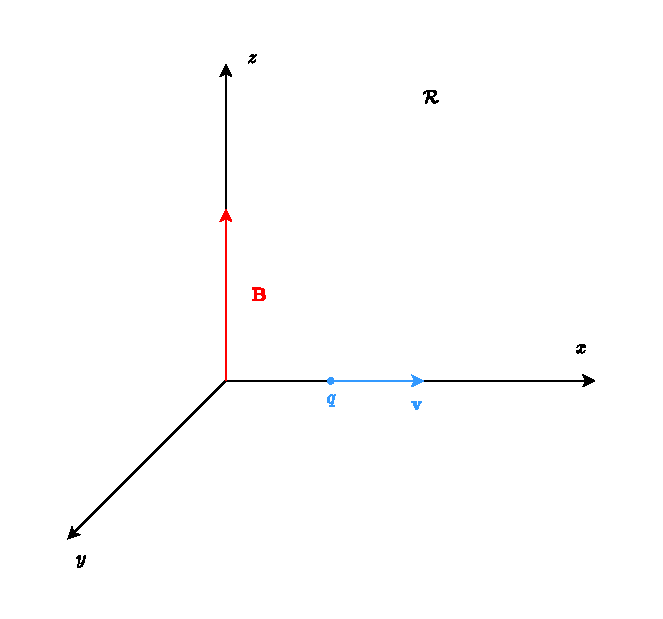
\includegraphics[width=0.6\linewidth]{res/svg/moving_particle_z_magnetic_irf1.drawio}
\end{figure}
In the first IRF a particle of charge $q$ and velocity $v$ along the $x$ axis feels a Lorentz force equal to:
\begin{equation}
  \vec{F} = q\brackets{\cancel{\vec{E}} + \vec{v} \cross \vec{B}} = -qv\hat{u}_yB_z
\end{equation}
In a new IRF $\irf{R}'$ where the particle is at rest the new fields are:
\begin{itemize}
  \item $\vec{E}' = \brackets{0,-\gamma v B_z,0}$
  \item $\vec{B}' = \brackets{0,0,\gamma B_z}$
\end{itemize}
\begin{figure}[H]
  \centering
  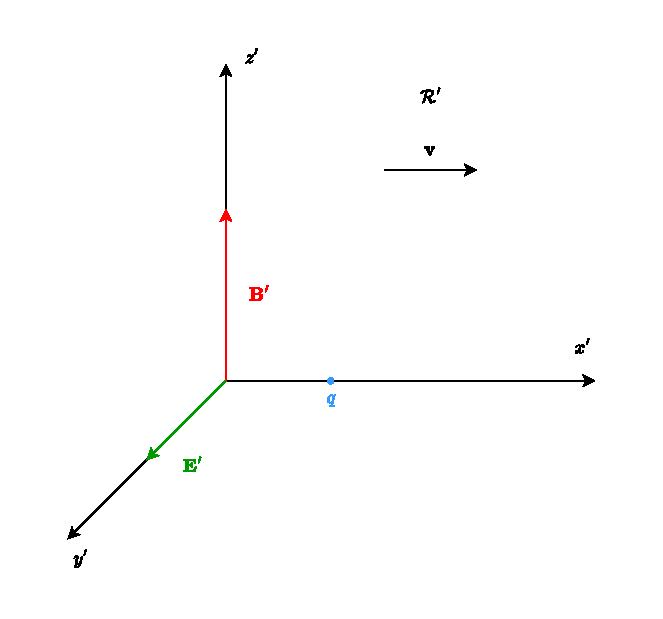
\includegraphics[width=0.6\linewidth]{res/svg/moving_particle_z_magnetic_irf2.drawio}
\end{figure}
And so the new Lorentz force is:
\begin{equation}
  \vec{F}' = q\brackets{\vec{E}' + \cancel{\vec{v}'\cross \vec{B}'}} = -q\gamma v B_z \hat{u}_y = \gamma \vec{F}
\end{equation}
And this is reasonable according to the general vector transformation equation of the force we got since:
\begin{equation}
  \begin{split}
    \vec{F}' &= \dfrac{\dfrac{\vec{F}}{\gamma (v)} + \vec{v}\sqbr{\brackets{1- \dfrac{1}{\gamma(v)}}\dfrac{\cancel{\vec{v}\cdot \vec{F}}}{v^2}-\dfrac{\cancel{\vec{F}\cdot \vec{u}}}{c^2}}}{1-\dfrac{\vec{v}\cdot\vec{u}}{c^2}} = \\[8pt]
    &= \dfrac{\dfrac{\vec{F}}{\gamma(v)}}{1-\dfrac{v^2}{c^2}} = \gamma(v)\vec{F}
  \end{split}
\end{equation}
Let's consider another example. A particle of charge $q$ is moving along a circular path with velocity $\vec{u}$ in a plane with a perpendicular magnetic field $\vec{B}$.
\begin{figure}[H]
  \centering
  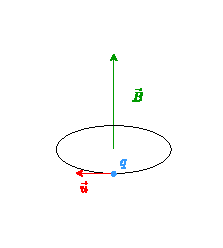
\includegraphics[width=0.6\linewidth]{res/svg/ciclotronic_motion.drawio}
\end{figure}
Since the particle is moving with a uniform circular motion $\norm{\vec{u}} = \text{constant}$. The Lorentz force acting on the particle is:
\begin{equation}
  \vec{F} = q\brackets{\cancel{\vec{E}} + \vec{u} \cross \vec{B}} = q\vec{u} \cross \vec{B}
\end{equation}
The magnitude of the force is thus $F = quB$ and the force is perpendicular to the velocity. Now we know that:
\begin{equation}
  F^{\mu} = m_0a^{\mu} = m_0 \gamma(u) \dv{}{t}\brackets{\gamma(u)c, \gamma(u)\vec{u}}
\end{equation}
Since $\gamma(u)$ is constant in time the 4-force becomes:
\begin{equation}
  F^{\mu} = m_0 \gamma^2(u)\brackets{0, \vec{a}}
\end{equation}
We also know that the 4-force can be expressed as:
\begin{equation}
  F^{\mu} = \brackets{\dfrac{\vec{F}\cdot \vec{u}}{c}, \vec{F}}
\end{equation}
And so for $\mu = 0$ we have:
\begin{equation}
  \vec{F}\cdot \vec{u} = 0
\end{equation}
This makes sense since the force is perpendicular to the velocity. Now we can compare the magnitude of the Lorentz force obtained through the electromagnetic relation $F = quB$ and the one obtained from the tensor relation:
\begin{equation}
  quB\cancel{\gamma(u)} = m_0\gamma^{\cancel{2}}(u)a
\end{equation}
And from this we can obtain $u$ knowing that $a = \dfrac{u^2}{R}$:
\begin{equation}
  \begin{split}
    &q\cancel{u}B = \dfrac{m_0\dfrac{u^{\cancel{2}}}{R}}{\sqrt{1-\dfrac{u^2}{c^2}}} \\[8pt]
    &\sqrt{1-\dfrac{u^2}{c^2}} = \dfrac{m_0u}{qBR} \\[8pt]
    &1-\dfrac{u^2}{c^2} = \dfrac{m_0^2u^2}{q^2B^2R^2} \\[8pt]
    &\dfrac{1}{u^2} = \dfrac{m_0^2}{q^2B^2R^2} + \dfrac{1}{c^2} \\[8pt]
    &\dfrac{1}{u^2} = \dfrac{m_0^2c^2 + q^2B^2R^2}{q^2B^2R^2c^2} \\[8pt]
    &\dfrac{1}{u^2} = \dfrac{m_0^2\cancel{c^2}\brackets{1 + \dfrac{q^2B^2R^2}{m_0^2c^2}}}{q^2B^2R^2\cancel{c^2}} \\[8pt]
    &\boxed{u = \dfrac{\dfrac{qBR}{m_0}}{\sqrt{1 + \dfrac{q^2B^2R^2}{m_0^2c^2}}}}
  \end{split}
\end{equation}
